\documentclass{article}
%\usepackage[francais]{babel}
%\usepackage[utf8]{inputenc} % Required for including letters with accents
%\usepackage[T1]{fontenc} % Use 8-bit encoding that has 256 glyphs
\usepackage{pythontex}
\usepackage{amsthm}
\usepackage{amsmath}
\usepackage{amssymb}
\usepackage{mathrsfs}
\usepackage{graphicx}
\usepackage{geometry}
\usepackage{stmaryrd}
\usepackage{tikz}
\usetikzlibrary{patterns}
%\usetikzlibrary{intersections}
\usepackage[cache=false]{minted}
\usepackage{xcolor}

\usepackage{stmaryrd}
%\usetikzlibrary{tikzmark}
\usepackage{empheq}
\usepackage{longtable}
\usepackage{booktabs} 
\usepackage{array}
\usepackage{pstricks}
\usepackage{pst-3dplot}
\usepackage{pst-tree}
\usepackage{pstricks-add}
\usepackage{upgreek}
%\usepackage{epstopdf}
\usepackage{eolgrab}
\usepackage{chngpage}
 \usepackage{calrsfs}
 % Appel du package pythontex 
\usepackage{pythontex}

\usepackage{algorithm2e}
\RestyleAlgo{algoruled}
  \SetKw{KwFrom}{from} 
\newenvironment{algo}{
\begin{algorithm}[H]
\DontPrintSemicolon \SetAlgoVlined}
{\end{algorithm}}



\usetikzlibrary{decorations.pathmorphing}
\def \de {{\rm d}}
\usepackage{color}
\usepackage{xcolor}
\newcommand{\mybox}[1]{\fbox{$\displaystyle#1$}}
\newcommand{\myredbox}[1]{\fcolorbox{red}{white}{$\displaystyle#1$}}
\newcommand{\mydoublebox}[1]{\fbox{\fbox{$\displaystyle#1$}}}
\newcommand{\myreddoublebox}[1]{\fcolorbox{red}{white}{\fcolorbox{red}{white}{$\displaystyle#1$}}}

\usepackage{xcolor}
%\setbeamercolor{background canvas}{bg=lightgray}
\definecolor{LightGray}{gray}{0.9}
\definecolor{monOrange}{rgb}{0.97,0.35,0.04}
\usepackage{enumitem}
 \title{Intéragir avec le DOM}
\author{Ibrahim ALAME}
\date{14/02/2023}
\begin{document}
\maketitle

\section{Introduction aux directives}
\subsection{Les directives}
Les directives sont des attributs spéciaux avec le préfixe {\color{monOrange}v-}. L'objectif d'une directive est d'appliquer de manière réactive des effets au {\tt DOM} lorsque la valeur de son expression change. Les directives natives sont les suivantes :
\begin{itemize}
\item v-text (qui équivaut à {{ }})
\item v-bind
\item v-html
\item v-once
\item v-show
\item v-if
\item v-else
\item v-else-if
\item v-for
\item v-on
\item v-model
\item v-pre
\item v-cloak
\item v-slot
\item v-memo
\end{itemize}

Il est également possible, comme nous l'étudierons, de créer ses propres directives {\color{monOrange}Vue}. Commençons par la directive la plus simple v-text.

\subsection{La directive {\color{monOrange}v-text} et l'interpolation de texte}
La directive {\color{monOrange}v-text} permet de mettre à jour le contenu de la propriété textContent de l'élément {\tt HTML}. La directive prend en argument la propriété déclarée sur le composant dont la valeur doit être utilisée. On appelle cela l'interpolation de texte. Par exemple, s'il existe une propriété message sur le composant dans la partie script, alors nous pouvons utiliser la directive de cette manière côté template :
\begin{minted}[
mathescape,
framesep=2mm,
baselinestretch=1.2,
fontsize=\footnotesize,
bgcolor=LightGray,
%linenos
]{html}
<span v-text="message"></span>
\end{minted}

La propriété {\color{blue}textContent} de l'élément {\tt span} sera alors remplacé par la valeur de la propriété {\tt message}. Comme lier une propriété est extrêmement courant, il existe une forme raccourcie appelée la notation moustache (de part sa forme), utilisant deux paires d'accolades :
\begin{minted}[
mathescape,
framesep=2mm,
baselinestretch=1.2,
fontsize=\footnotesize,
bgcolor=LightGray,
%linenos
]{html}
<span>{{message}}</span>
\end{minted}

Est du sucre syntaxique pour :
\begin{minted}[
mathescape,
framesep=2mm,
baselinestretch=1.2,
fontsize=\footnotesize,
bgcolor=LightGray,
%linenos
]{html}
<span v-text="message"></span>
\end{minted}

Note : en programmation, on appelle sucre syntaxique une syntaxe plus concise ou plus élégante qui est remplacée automatiquement par le code complet et donne le même résultat qu'une expression plus longue.

\subsection{Utilisation d'expression JavaScript}
Avec {\color{monOrange}Vue.js} il est possible d'utiliser toute expression {\tt JavaScript} valide comme argument d'une directive. Voici un exemple avec un ternaire :
\begin{minted}[
mathescape,
framesep=2mm,
baselinestretch=1.2,
fontsize=\footnotesize,
bgcolor=LightGray,
%linenos
]{javascript}
{{ condition ? 'Oui' : 'Non' }}
\end{minted}
Autre exemple :
\begin{minted}[
mathescape,
framesep=2mm,
baselinestretch=1.2,
fontsize=\footnotesize,
bgcolor=LightGray,
%linenos
]{javascript}
{{ message.reverse().toUpperCase() }}
\end{minted}

Encore un autre :
\begin{minted}[
mathescape,
framesep=2mm,
baselinestretch=1.2,
fontsize=\footnotesize,
bgcolor=LightGray,
%linenos
]{html}
<h1>Bonjour {{ `${prenom.toLowerCase()} ${nom.toUpperCase()}`}}</h1>
\end{minted}

Nous verrons énormément d'exemples au cours de la formation.

%Exemple exécutable
%Vous pouvez aussi directement utiliser ce code exécutable. N'hésitez pas à l'ouvrir dans un nouvel onglet :

\section{Directive {\color{monOrange}v-html}}
La directive {\color{monOrange}v-html} permet de mettre à jour l'attribut {\color{monOrange}innerHTML} d'un élément. Le contenu sera inséré comme du HTML simple.

Attention ! Le rendu dynamique de HTML sur votre site Web peut être très dangereux car il peut facilement conduire à des attaques {\tt XSS}. Utilisez uniquement {\color{monOrange}v-html} sur un contenu sûr et jamais sur du contenu fourni par l'utilisateur. Voici un exemple :
\begin{minted}[
mathescape,
framesep=2mm,
baselinestretch=1.2,
%fontsize=\footnotesize,
bgcolor=LightGray,
%linenos
]{html}
<p>Contenu HTML: <span v-html="varHtml"></span></p>
\end{minted}

%Exemple exécutable
%Vous pouvez aussi directement utiliser ce code exécutable. N'hésitez pas à l'ouvrir dans un nouvel onglet :

\section{Liaison de propriété avec v-bind}
La directive v-bind permet d'associer dynamiquement un attribut à une propriété.
\subsection{Syntaxe de base}
Elle prend en argument l'attribut auquel la propriété est liée. Ainsi par exemple :
\begin{minted}[
mathescape,
framesep=2mm,
baselinestretch=1.2,
%fontsize=\footnotesize,
bgcolor=LightGray,
%linenos
]{html}
<a v-bind:href="url"></a>
\end{minted}

L'attribut href de l'ancre est liée ici à la valeur de la variable url grâce à l'utilisation de la directive v-bind.

\subsection{Syntaxe raccourcie}
Comme cette directive est extrêmement utilisée, il existe une forme raccourcie :
\begin{minted}[
mathescape,
framesep=2mm,
baselinestretch=1.2,
%fontsize=\footnotesize,
bgcolor=LightGray,
%linenos
]{html}
<a :href="url"></a>
\end{minted}
C'est cette forme que nous utiliserons dans la formation et qui est recommandée.
\subsection{Utilisation sur des attributs booléens}
Les attributs booléens sont les attributs pour lesquels la simple présence de l'attribut représente la valeur true et leur absence la valeur false. Il y en a 26 différents.

Des exemples sont : disabled, checked, multiple, readonly, selected, hidden etc. Lorsque la directive v-bind est utilisée sur un attribut booléen, le comportement est le suivant : si la variable liée vaut true alors l'attribut sera ajouté par Vue.js automatiquement, si la variable vaut false alors l'attribut sera retiré. Par exemple :
\begin{minted}[
mathescape,
framesep=2mm,
baselinestretch=1.2,
%fontsize=\footnotesize,
bgcolor=LightGray,
%linenos
]{html}
<button :disabled="isButtonDisabled">Button</button>
\end{minted}

Si isButtonDisabled vaut true alors l'attribut disabled sera ajouté par Vue.js sur le DOM, s'il vaut false il sera enlevé.

\subsection{Utilisation sur plusieurs attributs}
La directive v-bind peut être utilisée pour lier un objet contenant des paires nom-valeur d'attribut. Exemple :
\begin{minted}[
mathescape,
framesep=2mm,
baselinestretch=1.2,
%fontsize=\footnotesize,
bgcolor=LightGray,
%linenos
]{html}
<div v-bind="{ id: propriété, 'autre-attribut': autrePropriété }"></div>
\end{minted}

Ainsi, si nous avons côté script :
\begin{minted}[
mathescape,
framesep=2mm,
baselinestretch=1.2,
%fontsize=\footnotesize,
bgcolor=LightGray,
%linenos
]{javascript}
const objet = {
  id: 'container',
  class: 'container'
}
\end{minted}

Nous pouvons lier cet objet avec la directive v-bind :
\begin{minted}[
mathescape,
framesep=2mm,
baselinestretch=1.2,
%fontsize=\footnotesize,
bgcolor=LightGray,
%linenos
]{html}
<div v-bind="objet"></div>
\end{minted}

Attention ! Dans ce cas la notation raccourcie n'est pas possible.
\subsection{Utilisation avec class et style}
Lorsqu'elle est utilisée avec les attributs class ou style, la directive v-bind peut prendre un tableau ou un objet en argument de cette façon :
\begin{minted}[
mathescape,
framesep=2mm,
baselinestretch=1.2,
%fontsize=\footnotesize,
bgcolor=LightGray,
%linenos
]{html}
<div :style="{ fontSize: size + 'px' }"></div>
\end{minted}
Ou :
\begin{minted}[
mathescape,
framesep=2mm,
baselinestretch=1.2,
%fontsize=\footnotesize,
bgcolor=LightGray,
%linenos
]{html}
<div :class="[classA, classB]"></div>
\end{minted}

Nous verrons des exemples dans la formation.

\subsection{Utilisation avec un attribut dynamique}
Vous pouvez utiliser une liaison dynamique également sur l'attribut avec cette syntaxe :
\begin{minted}[
mathescape,
framesep=2mm,
baselinestretch=1.2,
%fontsize=\footnotesize,
bgcolor=LightGray,
%linenos
]{html}
<button :[clé]="valeur"></button>
\end{minted}
Ici l'attribut peut être modifié dynamiquement en modifiant la valeur de la variable clé.

%Exemple exécutable
%Vous pouvez aussi directement utiliser ce code exécutable. N'hésitez pas à l'ouvrir dans un nouvel onglet :

\section{Utilisation de fonction dans les liaisons}
Comme nous l'avons vu, il est possible d'utiliser des expressions {\tt JavaScript} dans les templates. Nous pouvons donc invoquer des fonctions. Il est donc courant de voir :
\begin{minted}[
mathescape,
framesep=2mm,
baselinestretch=1.2,
%fontsize=\footnotesize,
bgcolor=LightGray,
%linenos
]{html}
<span :title="toTitleCase(titre)">
  {{ formatDate(date) }}
</span>
\end{minted}

Ici, nous utilisons deux invocations de fonction. L'une avec {\color{monOrange}v-bind} et l'autre avec {\color{monOrange}v-text}. Nous verrons de nombreux exemples au cours de la formation car c'est très courant.

%Exemple exécutable
%Vous pouvez aussi directement utiliser ce code exécutable. N'hésitez pas à l'ouvrir dans un nouvel onglet :

\section{Notions de base TypeScript}
\subsection{Les types statiques}
{\color{monOrange}TypeScript} permet de tout taper statiquement : vos variables, vos fonctions (arguments, valeur de retour) et vos classes. Le langage ne vous force pas à taper, ce qui vous laisse totalement libre de le faire ou non et ainsi d'adopter progressivement le typage statique en fonction de votre apprentissage.

\subsection{L'inférence de types}
{\color{monOrange}TypeScript}  va détecter automatiquement le type de votre variable en regardant la valeur qui lui est assignée. Nous reviendrons en détails sur cette fonctionnalité très pratique, mais elle permet sans aucune ligne supplémentaire d'avoir ce résultat :
\begin{minted}[
mathescape,
framesep=2mm,
baselinestretch=1.2,
%fontsize=\footnotesize,
bgcolor=LightGray,
%linenos
]{javascript}
const obj = { width: 1, height: 2 };
const aire = obj.width * obj.heigth;
// Property 'heigth' does not exist on type '{ width: number; height: number; }'. Did you mean // 'height'?
\end{minted}

Ici {\color{monOrange}TypeScript}  a détecté qu'aucune propriété {\tt heigth} n'existait sur objet vous invite à vérifier que vous n'avez pas fait une erreur. Magique, non ?

\subsection{Les types}
Comme son nom l'indique et comme nous l'avons vu {\color{monOrange}TypeScript}  est avant tout un langage pour taper. Il est possible de taper absolument tout comme nous le verrons : que ce soit les variables mais aussi les retours de fonction ou des situations encore plus complexes.

Typer au début peut sembler fastidieux : il faut ajouter un peu de code à chaque fois. Mais les bénéfices se remarquent très vite et dans cet ordre souvent :
\begin{enumerate}
\item  Vous aurez moins de bugs lors de l'exécution car beaucoup auront été signalés lors de la compilation : typo dans les noms, erreurs dans les conditions, dans les arguments passés, dans les retours de fonction etc.

\item   {\color{blue} VS} Code vous fournira avec un survol de la souris plein d'informations sur vos fonctions : quels arguments sont attendus etc, et vous gagnerez un temps fou grâce à l'autocomplétion (car  {\color{monOrange}TypeScript}  aura toutes les propriétés sur vos objets etc).

\item   Lorsque vous serez sur un projet à plusieurs, vous pourrez lire et comprendre beaucoup plus vite le code des autres développeurs car vous verrez facilement ce que prend et ce que retourne chaque fonction, quels sont les types acceptés par chaque variable etc.

\end{enumerate}
Une fois les premiers jours, où cela semblera être une surcouche embêtante, passée, vous ne pourrez plus faire sans !

\subsection{Les types primitifs}
Nous allons commencer par les types les plus basiques : les primitifs !

Pour préciser un type en  {\color{monOrange}TypeScript}  nous utilisons la plupart du temps (nous verrons en détails les autres cas) cette syntaxe :
\begin{minted}[
mathescape,
framesep=2mm,
baselinestretch=1.2,
%fontsize=\footnotesize,
bgcolor=LightGray,
%linenos
]{javascript}
variable: type;
\end{minted}

Il est possible de simplement taper une variable sans rien assigner ou de taper et assigner directement :
\begin{minted}[
mathescape,
framesep=2mm,
baselinestretch=1.2,
%fontsize=\footnotesize,
bgcolor=LightGray,
%linenos
]{javascript}
variable: type;
variable: type = x;
\end{minted}

\subsubsection{Les chaînes de caractères :string}
Les chaînes de caractères en {\color{monOrange}TypeScript}  comprennent exactement comme en {\tt JavaScript} les guillemets simples ou doubles et les accents graves ( {\tt backticks}) :
\begin{minted}[
mathescape,
framesep=2mm,
baselinestretch=1.2,
%fontsize=\footnotesize,
bgcolor=LightGray,
%linenos
]{javascript}
let prenom: string = "Jean";
prenom = 'Paul';
prenom = `Patrick`;
\end{minted}

\subsubsection{Les nombres :number}
Tous les nombres valides en {\tt JavaScript} le sont en {\color{monOrange}TypeScript} :
\begin{minted}[
mathescape,
framesep=2mm,
baselinestretch=1.2,
%fontsize=\footnotesize,
bgcolor=LightGray,
%linenos
]{javascript}
let decimal: number = 42;
let flottant: number = 42.22;
let hexadecimal: number = 0x2A;
let binaire: number = 0b101010;
let octal: number = 0o52;
\end{minted}

\subsubsection{Les booléens :boolean}
Le type {\tt boolean} n'accepte que {\tt true} ou {\tt false}:
\begin{minted}[
mathescape,
framesep=2mm,
baselinestretch=1.2,
%fontsize=\footnotesize,
bgcolor=LightGray,
%linenos
]{javascript}
let actif: boolean;
actif = true;
actif = false;
\end{minted}

\subsection{Le type any}
Il est possible de ne pas connaître le type de variables. Ces valeurs peuvent provenir d'un contenu dynamique, par exemple de l'utilisateur ou d'une bibliothèque tierce.

Il est également possible que vous souhaitiez taper plus tard votre fonction ou variable ou que vous soyez en train de convertir un fichier {\tt JavaScript} en {\color{monOrange}TypeScript} et que vous mettiez les types peu à peu.

Dans ces cas, nous souhaitons désactiver la vérification de type. Pour ce faire, nous les étiquetons avec le type {\color{blue}any}.
\begin{minted}[
mathescape,
framesep=2mm,
baselinestretch=1.2,
%fontsize=\footnotesize,
bgcolor=LightGray,
%linenos
]{javascript}
let pasSur: any = 4;
pasSur = 'en fait une string';
\end{minted}

Lorsque vous commencez en {\color{monOrange}TypeScript} vous aurez tendance à beaucoup trop utiliser {\color{blue} any}. A chaque fois que vous ne saurez pas trop le type vous mettrez {\color{blue} any}. Au début ce n'est pas très grave mais il faut vous forcer à faire l'effort de tout bien typer pour garder les bénéfices de l'usage de  {\color{monOrange}TypeScript}. Nous vous recommandons de ne quasiment jamais utiliser {\color{blue} any} sauf dans les cas vus ci-dessus.

\subsection{Le type {\color{monOrange}object}}
Le type {\color{monOrange}objet} permet simplement de représenter le type {\color{blue}non primitif} : tout ce qui n'est pas {\tt number, string, boolean, bigint, symbol, null} ou {\tt undefined}. Cela peut donc être un tableau, un objet littéral, etc.
\begin{minted}[
mathescape,
framesep=2mm,
baselinestretch=1.2,
%fontsize=\footnotesize,
bgcolor=LightGray,
%linenos
]{javascript}
let monObj: object;
monObj = {};
\end{minted}

Notez que {\color{monOrange}object} et {\color{monOrange}{}} sont deux manières de typer un objet, nous pouvons écrire :
\begin{minted}[
mathescape,
framesep=2mm,
baselinestretch=1.2,
%fontsize=\footnotesize,
bgcolor=LightGray,
%linenos
]{javascript}
let monObj: {};
monObj = {};
\end{minted}

\subsection{Le type {\color{monOrange}array}}
Il y a deux syntaxes en {\tt TypeScript} pour taper les {\color{monOrange}tableaux} . En {\tt TypeScript} un tableau est un tableau {\tt JavaScript} contenant un nombre indéfini d'éléments . Première possibilité :
\begin{minted}[
mathescape,
framesep=2mm,
baselinestretch=1.2,
%fontsize=\footnotesize,
bgcolor=LightGray,
%linenos
]{javascript}
type[];
\end{minted}

Où type est le type des éléments contenus dans un tableau. Il est possible d'accepter par exemple que les nombres :
\begin{minted}[
mathescape,
framesep=2mm,
baselinestretch=1.2,
%fontsize=\footnotesize,
bgcolor=LightGray,
%linenos
]{javascript}
let liste: number[] = [1, 2, 3];
\end{minted}
Tous les types :
\begin{minted}[
mathescape,
framesep=2mm,
baselinestretch=1.2,
%fontsize=\footnotesize,
bgcolor=LightGray,
%linenos
]{javascript}
let liste: any[] = [1, true, {}];
\end{minted}

\subsection{Qu'est-ce qu'une {\color{monOrange}interface} ?}
Une {\color{monOrange}interface} est un contrat qui définit la forme qui doit prendre un objet {\tt JavaScript} (objets littéraires, classes et fonctions) . Il est important de noter qu'une {\color{monOrange}interface} n'est pas compilée : aucun code {\tt JavaScript} ne sera créé à partir de l'interface. Elle sert uniquement pour l' IDE, c'est-à-dire pour {\color{blue}VS Code}, (auto-complétions et erreurs de types) et lors de la compilation.

\subsubsection{Notre première interface}
Prenons un premier exemple avec un objet :
\begin{minted}[
mathescape,
framesep=2mm,
baselinestretch=1.2,
%fontsize=\footnotesize,
bgcolor=LightGray,
%linenos
]{javascript}
interface User {
    prenom: string;
}
\end{minted}

Ici, notre objet {\color{monOrange}User} doit obligatoirement avoir une propriété {\color{blue}prenom} contenant une chaîne de caractères. Ensuite nous pouvons utiliser l' interface pour taper par exemple un paramètre d'une fonction :
\begin{minted}[
mathescape,
framesep=2mm,
baselinestretch=1.2,
%fontsize=\footnotesize,
bgcolor=LightGray,
%linenos
]{javascript}
function printUser(user: User) {
    console.log(user.prenom);
}
\end{minted}

Ici, la fonction {\color{blue}printUser} doit recevoir en argument un objet respectant l' interface {\color{monOrange}User} . Par exemple :
\begin{minted}[
mathescape,
framesep=2mm,
baselinestretch=1.2,
%fontsize=\footnotesize,
bgcolor=LightGray,
%linenos
]{javascript}
let paul = {prenom: 'Paul'};
printUser(paul);
\end{minted}

Attention ! Lorsque vous tapez le paramètre de cette manière {\tt user: User} , cela revient à dire que le paramètre doit au moins avoir le ou les propriétés de l'interface {\color{blue}User} et donc avoir une propriété {\tt prenom}.

En revanche, lorsque vous tapez un objet avec une interface, il faut que l'objet respecte exactement l'interface . C'est-à-dire qu'il doit avoir exactement les propriétés définies, ni plus ni moins. Voici un exemple pour bien comprendre :
\begin{minted}[
mathescape,
framesep=2mm,
baselinestretch=1.2,
%fontsize=\footnotesize,
bgcolor=LightGray,
%linenos
]{javascript}
interface User {
    prenom: string;
}

function printUser(user: User) {
    console.log(user.prenom);
}

const paul = {prenom: 'Paul', nom: 'Dupont'};

printUser(paul); // Cela fonctionne car paul a au moins une propriété nom

const jean: User = {prenom: 'Jean', nom: 'Duprey'}; // Erreur
\end{minted}

Dans le cas de l'objet {\color{blue} Jean}, {\tt TypeScript} nous signalons l'erreur suivante : {\bf Type '{ prenom: string; nom: string; }' is not assignable to type 'User'. Object literal may only specify known properties, and 'nom' does not exist in type 'User'}.

Autrement dit, il se plaint car {\color{blue} Jean} a une propriété {\tt nom} qui ne respecte pas le contrat imposé par l' interface {\color{monOrange} User}.

\subsubsection{Les propriétés optionnelles avec?}
Il est possible de définir des propriétés optionnelles comme nous l'avons vu pour les arguments de fonction en utilisant {\color{monOrange} ?}. Ces propriétés sont également utilisables dans les interfaces.
\begin{minted}[
mathescape,
framesep=2mm,
baselinestretch=1.2,
%fontsize=\footnotesize,
bgcolor=LightGray,
%linenos
]{javascript}
interface User {
  prenom: string;
  nom?: string;
}
\end{minted}

Ici, nous établissons comme contrat que les objets qui respecteront l' {\color{monOrange}interface User} auront obligatoirement une propriété {\tt prenom} contenant une chaîne de caractères, et une propriété optionnelle {\tt nom}, qui si elle existe, devra également contenir une chaîne de caractères. En outre, les propriétés optionnelles permettent l'autocomplétion et l'autocorrection.

\subsection{Les unions de type}
Les unions de type permettent de combiner deux ou plusieurs types et s'utilisent avec {\color{monOrange}|} . Les unions s'utilisent dans toutes les situations.

\subsubsection{Unions de type et variables}
Prenons un premier exemple :
\begin{minted}[
mathescape,
framesep=2mm,
baselinestretch=1.2,
%fontsize=\footnotesize,
bgcolor=LightGray,
%linenos
]{javascript}
let uneVar: string | number;}
\end{minted}

Ici, nous effectuons une union entre les types de chaîne de caractères et de nombres. La variable pourra ainsi recevoir l'un des deux types.

\subsubsection{Unions de type et fonctions}
Vous pouvez également taper les paramètres des fonctions en utilisant des unions :
\begin{minted}[
mathescape,
framesep=2mm,
baselinestretch=1.2,
%fontsize=\footnotesize,
bgcolor=LightGray,
%linenos
]{javascript}
function ajouter(a: string | number, b: string | number) {
  return Number(a) + Number(b);
}
\end{minted}

Ici par exemple, notre fonction peut ajouter des nombres et des chaînes de caractères. Nous voulons donc utiliser des unions pour les paramètres de la fonction. Vous pouvez également taper les retours de fonctions en utilisant des unions :
\begin{minted}[
mathescape,
framesep=2mm,
baselinestretch=1.2,
%fontsize=\footnotesize,
bgcolor=LightGray,
%linenos
]{javascript}
function ajouter(isAdmin: boolean): string | void {
  if (isAdmin) {
    return 'secret';
  } else {
    return;
  }
}
\end{minted}


%Exemple exécutable
%Vous pouvez également utiliser directement ce code exécutable. N'hésitez pas à l'ouvrir dans un nouvel onglet :

\section{Les événements natifs}
\subsection{La gestion des événements}
L'objectif de la gestion des événements est de pouvoir réagir à un évènement. Les événements HTML sont des événements qui se produisent suite aux interactions de l'utilisateur avec son clavier, sa souris ou alors à la modification d'éléments du DOM:
\begin{itemize}
\item {\em modification de l'objet {\color{monOrange}window}} : par exemple la page est fini d'être chargé
\item {\em modification d'un formulaire }: par exemple lorsqu'un champion est invalide
\item {\em interactions clavier ou souris }: par exemple une pression de toucher
\item {\em événements relatifs à un média (vidéo, audio) }: par exemple lorsqu'une vidéo finie
\item {\em événements relatifs au glisser-déposer }: par exemple lorsqu'un élément a été glissé
\end{itemize}

Lorsqu'il {\color{monOrange}Vue.js} est appliqué sur une page, HTML il peut réagir à ces événements.

\subsubsection{L'approche de {\color{monOrange}Vue.js}}
Dans {\color{monOrange}Vue.js} les écouteurs sont déclarés dans le HTML. Pourquoi cette approche ?
\begin{enumerate}
\item  permet de voir directement dans le HTML où se situent les écouteurs d'événement et à quel élément ils sont attachés.
\item  permet de ne pas avoir à mettre des sélecteurs et des écouteurs latéraux JavaScript offrant ainsi la possibilité de n'avoir que la logique dans le JavaScript et de pouvoir mieux tester.
\item  Lorsqu'un composant est détruit, tous les écouteurs sont également retirés automatiquement.
\end{enumerate}

\subsubsection{{\color{monOrange}v-on}: écouter des événements du DOM}
La directive {\color{monOrange}v-on} permet d'écouter des événements et d'attacher un gestionnaire d'événement à un évènement . Le type d'événement est déterminé par l'argument qui est passé à {\color{monOrange}v-on}, ainsi par exemple : {\tt v-on:keyup} permet d'écouter l'événement du relâchement d'une touche du clavier.

\subsubsection{Le raccourci@}
{\color{monOrange}v-on} peut être remplacé par un raccourci : {\color{monOrange}@}.
\begin{minted}[
mathescape,
framesep=2mm,
baselinestretch=1.2,
%fontsize=\footnotesize,
bgcolor=LightGray,
%linenos
]{html}
<button @click="direBonjour">Dire bonjour</button>
\end{minted}

Ici un {\color{monOrange}clic} sur le bouton va déclencher la fonction {\tt direBonjour()} du composant. Autrement dit, l'événement {\color{monOrange}click} va exécuter le gestionnaire d'événement {\tt direBonjour()}.

\subsubsection{L'objet {\color{monOrange}event} reçu}
Le gestionnaire d'événement reçoit automatiquement l'événement du DOM en argument . Par exemple :
\begin{minted}[
mathescape,
framesep=2mm,
baselinestretch=1.2,
%fontsize=\footnotesize,
bgcolor=LightGray,
%linenos
]{html}
<template>
  <button @click="direBonjour">Dire bonjour</button>
</template>

<script setup lang="ts">
function direBonjour(event: MouseEvent)
{
    console.log(event);
}
</script>
\end{minted}
Notez que nous typons l'événement comme un {\color{monOrange}MouseEvent} pour pouvoir accéder à toutes les propriétés et méthodes par autocomplétion.

\subsubsection{Passer un argument à un gestionnaire d'événement}
Notez que vous pouvez passer un argument à un gestionnaire d'événement, dans ce cas l'événement sera disponible en deuxième argument . Il faut passer {\color{monOrange}\$event} en deuxième argument au gestionnaire d'événement pour pouvoir y accéder dans la fonction :
\begin{minted}[
mathescape,
framesep=2mm,
baselinestretch=1.2,
%fontsize=\footnotesize,
bgcolor=LightGray,
%linenos
]{html}
<template>
  <button @click="direBonjour('Salut', $event)">Dire bonjour</button>
</template>

<script setup lang="ts">
function direBonjour(arg: string, event: MouseEvent)
{
    console.log(arg);
    console.log(event);
}
</script>
\end{minted}

\subsection{L'assertion {\color{monOrange}TypeScript} avec {\color{monOrange}as}}
Dans certains cas, vous aurez besoin de signaler {\color{monOrange}TypeScript} que vous êtes sûr d'un type et qu'il n'a pas à s'en préoccuper. Autrement dit, vous lui désignez un type et vous l'obligez à le respecter, c'est ce qu'on appelle l'assertion. L'assertion doit être manipulée avec prudence car vous perdez le bénéfice du contrôle de type avant l'exécution. Pour l'assertion il faut utiliser :
\begin{minted}[
mathescape,
framesep=2mm,
baselinestretch=1.2,
%fontsize=\footnotesize,
bgcolor=LightGray,
%linenos
]{javascript}
as type
\end{minted}
Par exemple :
\begin{minted}[
mathescape,
framesep=2mm,
baselinestretch=1.2,
%fontsize=\footnotesize,
bgcolor=LightGray,
%linenos
]{javascript}
let maVar: any = "Une chaîne";

let longueur: number = (maVar as string).length;
\end{minted}
Ici nous avons forçons {\color{monOrange}TypeScript} à reconnaître {\tt maVar} comme étant une chaîne de caractères pour pouvoir utiliser l'autocomplétion et la propriété {\tt length}. Le plus souvent nous souhaitons utiliser une interface HTML comme dans la vidéo, afin d'obtenir les bonnes propriétés et les bonnes méthodes. En effet, TypeScriptne peut pas connaître l'élément du DOM HTML et il faut donc le lui préciser. Vous verrez donc asla plupart du temps dans ce cas.

%Exemple exécutable
%Vous pouvez également utiliser directement ce code exécutable. N'hésitez pas à l'ouvrir dans un nouvel onglet :


%%%%%%%%%%%%%%%%%%%%%%%%%%%%%%%%%%%%%%%%%%%%%%%%%%%%%%%%%%%%%%
\section{Les modificateurs d'événements}
\subsection{Les modificateurs d'événements ( {\color{monOrange}event modifiers})}
Les modificateurs d'événements permettent de modifier des événements avant qu'ils soient gérés dans les gestionnaires d'événements. Ils sont très pratiques pour deux raisons : premièrement, ils permettent aux gestionnaires de ne s'occuper que de la logique et deuxièmement, de raccourcir et simplifier la syntaxe. {\color{monOrange}Vue.js} proposer huit modificateurs d'évènements :
\begin{itemize}
\item {\color{blue} .stop}: {\tt verserevent.stopPropagation()}
\item {\color{blue} .prevent} {\tt  event.preventDefault()}
\item {\color{blue} .self} pour ne déclencher l'événement que s'il est envoyé de cet élément
\item {\color{blue} .once} pour ne déclencher l'événement qu'une seule fois
\item {\color{blue} .passive} pour ajouter {\tt le mode passif}
\item {\color{blue} .capture} pour ajouter l'écouteur d'événement en mode {\tt capture}
\end{itemize}
Il s'utilise de cette manière :
\begin{minted}[
mathescape,
framesep=2mm,
baselinestretch=1.2,
%fontsize=\footnotesize,
bgcolor=LightGray,
%linenos
]{html}
<button type="submit" @click.prevent="calculer">Calculer</button>
\end{minted}

\subsection{Touches de contrôle ( {\color{monOrange}key modifiers})}
{\color{monOrange}Vue.js} facilite grandement la gestion des événements claviers et souris, il fournit ainsi de nombreuses méthodes afin de réagir à ces événements. Par exemple pour réagir à la touche entrée :
\begin{minted}[
mathescape,
framesep=2mm,
baselinestretch=1.2,
%fontsize=\footnotesize,
bgcolor=LightGray,
%linenos
]{html}
<input @keyup.13="submit"> // en utilisant le code de la touche
<input @keyup.enter="submit"> // en utilisant l’alias proposé par Vue
\end{minted}
La liste des alias proposés par Vue pour le clavier est la suivante :
\begin{itemize}
\item {\color{blue} .enter}
\item {\color{blue} .tab}
\item {\color{blue} .delete}
\item {\color{blue} .esc}
\item {\color{blue} .space}
\item {\color{blue} .up}
\item {\color{blue} .down}
\item {\color{blue} .left}
\item {\color{blue} .right}
\item {\color{blue} .ctrl}
\item {\color{blue} .alt}
\item {\color{blue} .shift}
\item {\color{blue} .meta}( (équivaut à cmd ou touche windows) )
\end{itemize}
Pour la souris :
\begin{itemize}
\item {\color{blue} .left}
\item {\color{blue}.right}
\item {\color{blue}.middle}
\end{itemize}
Exemple exécutable
Vous pouvez également utiliser directement ce code exécutable. N'hésitez pas à l'ouvrir dans un nouvel onglet :

\end{document}

\begin{center}
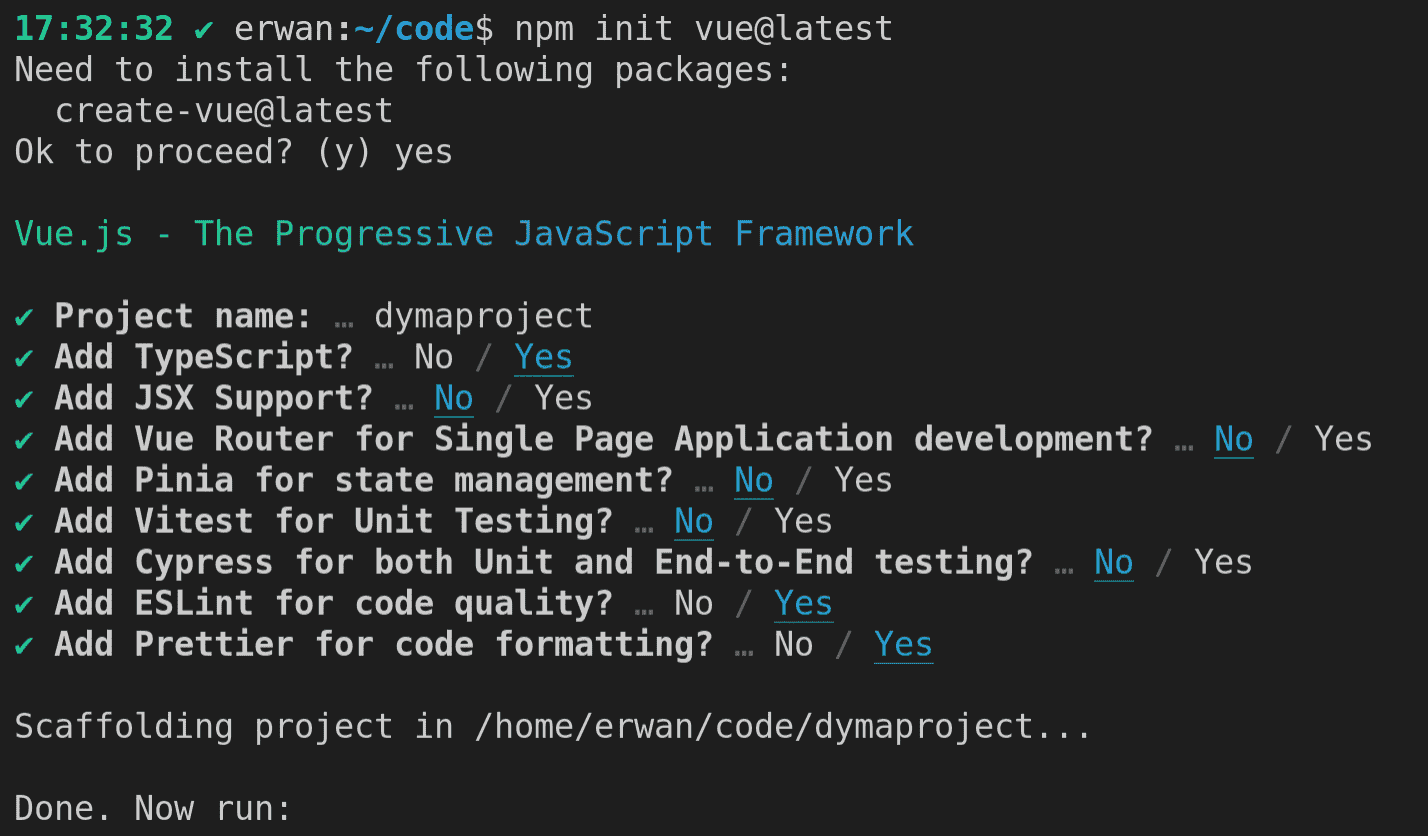
\includegraphics[width=10cm]{images/image04.png}
\end{center}


\end{document}

